%latex model.tex
%bibtex model
%latex model.tex
%latex model.tex
%pdflatex model.tex

%se poate lucra si online (de ex www.overleaf.com)


\documentclass[runningheads,a4paper,11pt]{report}

\usepackage{algorithmic}
\usepackage{algorithm} 
\usepackage{array}
\usepackage{amsmath}
\usepackage{amsfonts}
\usepackage{amssymb}
\usepackage{amsthm}
\usepackage{caption}
\usepackage{comment} 
\usepackage{epsfig} 
\usepackage{fancyhdr}
\usepackage[T1]{fontenc}
\usepackage{geometry} 
\usepackage{graphicx}
\usepackage[colorlinks]{hyperref} 
\usepackage[latin1]{inputenc}
\usepackage{multicol}
\usepackage{multirow} 
\usepackage{rotating}
\usepackage{setspace}
\usepackage{subfigure}
\usepackage{url}
\usepackage{verbatim}
\usepackage{xcolor}
\usepackage{listings}
\usepackage{tabularx}


\geometry{a4paper,top=3cm,left=2cm,right=2cm,bottom=3cm}
\graphicspath{ {./images/} }

\pagestyle{fancy}
\fancyhf{}
\fancyhead[LE,RO]{Pedestrians Detector}
\fancyhead[RE,LO]{Team's name}
\fancyfoot[RE,LO]{ITSG 2021-2022}
\fancyfoot[LE,RO]{\thepage}

\renewcommand{\headrulewidth}{2pt}
\renewcommand{\footrulewidth}{1pt}
\renewcommand{\headrule}{\hbox to\headwidth{%
  \color{lime}\leaders\hrule height \headrulewidth\hfill}}
\renewcommand{\footrule}{\hbox to\headwidth{%
  \color{lime}\leaders\hrule height \footrulewidth\hfill}}

\hypersetup{
pdftitle={artTitle},
pdfauthor={name},
pdfkeywords={pdf, latex, tex, ps2pdf, dvipdfm, pdflatex},
bookmarksnumbered,
pdfstartview={FitH},
urlcolor=cyan,
colorlinks=true,
linkcolor=red,
citecolor=green,
}
% \pagestyle{plain}

\setcounter{secnumdepth}{3}
\setcounter{tocdepth}{3}

\linespread{1}

% \pagestyle{myheadings}

\makeindex


\begin{document}

\begin{titlepage}
\sloppy

\begin{center}
BABE\c S BOLYAI UNIVERSITY, CLUJ NAPOCA, ROM\^ ANIA

FACULTY OF MATHEMATICS AND COMPUTER SCIENCE

\vspace{6cm}

\Huge \textbf{PEDESTRIANS DETECTOR}

\vspace{1cm}

\normalsize -- MIRPR report --

\end{center}


\vspace{5cm}

\begin{flushright}
\Large{\textbf{Team members}}\\
Name, specialisation, group, email
\end{flushright}

\vspace{4cm}

\begin{center}
2021-2022
\end{center}

\end{titlepage}

\pagenumbering{gobble}

\begin{abstract}
	Text of abstract. Short info about: 
	\begin{itemize}
		\item project relevance/importance, 
		\item inteligent methods used for solving, 
		\item data involved in the numerical experiments; 
		\item conclude by the the results obtained.
	\end{itemize}

	Please add a graphical abstract of your work. 
\end{abstract}


\tableofcontents

\newpage

\listoftables
\listoffigures
\listofalgorithms

\newpage

\setstretch{1.5}



\newpage

\pagenumbering{arabic}


 


\chapter{Introduction}
\label{chapter:introduction}

\section{What? Why? How?}
\label{section:what}


There are a lot of people out there dreaming about how the future will look like, and there is a very common answer to this question: self-driving cars. Currently, the automotive industry is trying to step out of the ordinary and offer an autonomous experience to the driver. A car is equipped with lots of sensors, just like humans - it can see things, or react to them. The idea is to teach the car to make decisions based on what these sensors intercept. This paper is trying to focus on one of the many branches of autonomous driving: endowing the car with the ability of seeing.
\begin{itemize}
	\item What is the (scientific) problem? 
	
	An autonomous car should be able to "see" and make its own decisions based on the input. This paper aims to provide a fast and reliable computer vision solution for pedestrians detection, which is one of the most crucial aspects when it comes to self-driving cars. Using the input from the camera, any pedestrian should be detected in less than the blink of an eye, and from a considerable distance, so that the moving car gets the possibility to react smoothly.
	\item Why is it important? 
	
	The goal is to get to a higher level of autonomy, but the hardest thing to do is keeping humans as safe as possible. The number of car crashes is huge every year, mostly because of lack of attention or driver's drowsiness. A machine will never get tired and this is why the automotive industry is trying to design the car to take over most of the driver's responsibilities. The thing here is that when it comes to human safety, the machine is not allowed to make mistakes, so the purpose is first of all to make these detection algorithms reach perfection.
	  
	\item What is your basic approach? 
	
	The idea is to create an intelligent algorithm that gets an image as input and outputs it with an emphasis on where the pedestrian has been detected. The algorithm should be able to provide really fast and accurate responses, therefore transfer learning techniques will also be used.  
\end{itemize}



\section{Paper structure and original contribution(s)}
\label{section:structure}

The research presented in this paper is focused on outlining the theory behind the TinyYoloV3 model and employing it for the particular problem of pedestrian detection in different contexts.

The main contribution of this report is to present a solution based on an intelligent classifier consisting of a pre-trained model which is run against multiple sets of data in the aim of solving the problem of pedestrian, vehicle and road sign detection.

The second contribution of this report is the development of a simple and intuitive mobile application that will present a practical user interface through which the user can easily test the algorithm results on input of their own.

The third contribution of this thesis consists of the employment of a number of optimizations with a view to increasing the overall accuracy of the algorithm and testing its performance in different scenarios.

The work is structured in seven chapters as follows: 

The first chapter is a short introduction in the subject of object detection in the driving assistance field, what it is about and why it is important and our reasons that were behind choosing this topic. 

The second chapter describes the scientific problem in more detai and considers the advantages and disadvantages of our aproachl.

The third chapter treats some other related work in the field and gives a brief description of their results.

In chapter four we provide the investigate approach, togheter with the tools and technologies that were used in order to implement it. We describe the underlying architecture of the TinyYoloV3 model and the algorithm employed by it, stating how we will use this for our problem and how it is suited for the driving assistance object of study. We show how the algorithm works in practice and provide a short list of the tools we will be using for our study.

Chapter five comprises the main part of this report and consists of the description of our application requirements, the methodology by which we plan to solve the problem, the datasets we will be conducting our experiments on and the results obtained in the end. At the end of the chapter, we also provide some discussion around the results and potential optimizations to the algorithm, comparing the results obtained with the initial ones. The chapter ends with a small presentation of the user interface.

Chapter 6 explains the experimental methodology and the numerical results obtained with our approach and the state of the art approaches. Our focus in this chapter is on the interpretation and the statistical validation of the results. Also, this chapter is a dive into the philosophical aspects of autonomous driving and how this is likely to affect the way in which we report ourselves to the task of driving in general. We analyze the objectivity of the solution proposed and raise some interesting questions relating to the ethics of the smart driving assistants in general. We also provide some interesting data about the way our algorithm performs on individuals of different races and ethnicities, by this trying to advance the idea of diversity and inclusion in the way we use such technology.

The last chapter offers a summarization of our conclusions and future work and also try to analyze the strenghts and weaknesses of our application with the focus on what we can improve both in the algorithm and the application.



\chapter{Scientific Problem}
\label{section:scientificProblem}


\section{Problem definition}
\label{section:problemDefinition}

Advanced driver-assistance systems (ADAS) are groups of electronic technologies that assist drivers in driving and parking functions. Through a safe human-machine interface, ADAS increase car and road safety. ADAS use automated technology, such as sensors and cameras, to detect nearby obstacles or driver errors, and respond accordingly.

As most road accidents occur due to human error, ADAS are developed to automate, adapt, and enhance vehicle technology for safety and better driving. ADAS are proven to reduce road fatalities by minimizing human error. Safety features are designed to avoid accidents and collisions by offering technologies that alert the driver to problems, implementing safeguards, and taking control of the vehicle if necessary. Adaptive features may automate lighting, provide adaptive cruise control, assist in avoiding collisions, incorporate satellite navigation and traffic warnings, alert drivers to possible obstacles, assist in lane departure and lane centering, provide navigational assistance through smartphones, and provide other features.

The point of this paper is to show a implies of identifying people on foot in any kind of conditions and tie this to the current climate state to propose to the client the foremost suitable activities to be taken in certain activity circumstances or to respond naturally to them.

The main advantage of an artificial intelligent algorithm is its ability to analyse and employ an enormous quantity of data, much more efficiently than possible for humans through classical statistical analyses. Moreover, the more data received, the more accurate the result will be.

The personal driving assistant would be built off an intelligent classification algorithm based on neural networks. Other methods used for obstacle detection include:
\begin{itemize}
	\item template matching approach - the real image is compared against a sufficient number of templates of the object-of-interest to identify the presence of the object in the sample image.
\end{itemize}

We will be using the Deep Learning approach. Our classifier will receive as input the image or video sequence and output the same image, with the obstacles marked and delimited accordingly. This should provide a good start for further improvements and additional features that would contribute to a better navigation experience in autonomous driving.

On the other hand, processing image with people is a challenge even for an intelligent algorithm. Most of the images may be difficult to read an interpret, which means that large sets of data with labeled images are required for the algorithm to work properly. Machines are still having a hard time understanding images with people and using certain unclear images can be misleading for the AI, that can provide erroneous or implausible detections.

\section{Challenges}

Much of effort was concentrated on trying to make the algorithm run faster and get a better accuracy with the amount of resources that we have had at our disposal. In trying to work with a model that is pre-trained, we have had little control over the time it takes the algorithm to do a detection. The models themselves are pretty large in size and take up a great deal of resources to run. 

Lack of sufficient resources to run the algorithm was an imminent problem that we have come across.



\chapter{State of the art/Related work}
\label{chapter:stateOfArt}

In this chapter we present a few methods that were used for pedestrian detection in different contexts. In order to provide safety and to reduce traffic accidents driving assistance systems have been developed with the help of artificial intelligence and ones of the features are pedestrian detectors and driving assistants.

Firstly, we will take a look at "Traffic signs recognition for driving assistance" (add link to bibliography) by Yatham Sai Sangram Reddy, Devareddy Karthik, Nikunj Rana, M Jasmine Pemeena Priyadarsini, G K Rajini
and Shaik Naseera.
\begin{itemize}
	\item What is their problem and method?
	
	Problem: The paper proposes a method to detect the traffic sign board in a frame and to identify the sign on it. 
	
	Used algorithm: HAAR Cascade Training - Viola Jones Algorithm for detecting differences in pixel intensities.
	\item How is our problem and method different? 
	
	Our problem is a little bit different than the one from the mentioned paper, because we try to detect people that are present in certain picture. At the same time, they mention using real-time camera system. The implementation is also done differently, since we are using COCO-SSD for object detection, while their implementation was done by training a cascade classifier for head detection from the scene, by using HAAR features through OpenCV.
	\item DataSets: Each of the Traffic signs is recognised using a database of images of numbers and symbols used to train the KNN classifier using OpenCV libraries. The images are split into positives (containing the target road sign) and negatives (containing background). For each positive image an annotation file is created, and then a vector (.vec) file for all of them.
	\item Results: For the traffic signs with single contours, the nearest neighbour is found and the output is the response returned by the classifier. For the traffic signs with multiple contours, the responses returned by the classifier are sorted based on their x-positions after the
    nearest neighbours are found. The authors do not offer an aggregated result in terms of accuracy or detection rate of their algorithm. Some sample outputs are presented, though, and they look like: "Sign Board: School Zone", "Speed limit: 50 km/h" etc. The algorithm works directly on frames captured from the camera and presents satisfactory results.
    
\end{itemize}

    Next, we will take a look at "Driving situation-based real-time interaction with intelligent driving assistance agent" (add link to bibliography) by Young-Hoon Nho.
    \begin{itemize}
	\item What is their problem and method?
	
	Problem: The article presents an intelligent driving assistance agent that interacts with the driver in real time. Different driving situations are recognized by the algorithm, such as speed bump, corner, crowded area, uphill, downhill, straight, parking space. The algorithm combines driving intention recognition with driving situation information, that is automatically tagged as the vehicle is driven, to build a long-term interaction model.
	
	Used algorithm: They use an algorithm based on hidden Markov models (HMMs).
	\item How is our problem and method different? 
	
	Our problem is a little bit different than the one from the mentioned paper, because we try to detect people that are present in certain picture. At the same time, they mention using real-time camera system. The implementation is also done differently, since we are using COCO-SSD for object detection, while their implementation was done by using an algorithm based on hidden Markov models.
	\item DataSets: The acquisition of data was done in intervals, while driving a Kia Morning vehicle, using on-board diagnostics 2 (OBD2). The data collected included: steering wheel data, velocity and accelerator pedal data, latitude and longitude as serial data. 430 data inputs were obtained, each of them being labeled by one of the 7 driving situations considered.
	\item Results: The results they obtained with this approach is 94.9% accuracy, more specifically - 408 our of 430 correctly recognized inputs.
    
\end{itemize}



\chapter{Investigated approach}
\label{chapter:proposedApproach}

% \section{Motivation}
% \label{section:motivation}

There are a lot of documented ways of implementing object detection nowadays, and most of them are written in Python. Why is this the most popular language for AI and ML based projects? Because it offers a great library ecosystem. Libraries provide base level items so developers don't have to code them from the beginning every time.
(https://djangostars.com/blog/why-python-is-good-for-artificial-intelligence-and-machine-learning/)

TensorFlow is a free and open-source library for machine learning and artificial intelligence. It can be used across a range of tasks but has a particular focus on training and inference of deep neural networks. It uses Python to provide a convenient front-end API for building applications, while executing those applications in high-performance C++. This is the core library that is used in this project, with a twist that will be revealed in the second experiment.

\section{First Experiment}
\label{section:firstExperiment}

We first started by implementing a mobile application with a regular client-server model. The server was written in Python with a Flask RESTful API. The client side is implemented in React Native and has to send the photo to the server and then wait for the detection. 

The YOLOv3 pre-trained model we have decided to use comes with vehicle, persons and road sign detection out of the box, so we only need to fine-tune it to fit the specific needs of our application and optimize its performance for our problem.

The way we will measure the quality of the detection is by tracking the overall accuracy and trying to maximize the number of successful detections, at the same time reducing the number of false positives. Another aspect that we considered of tremendous importance is the speed of the algorithm, since we are striving for a pleasant user experience and are driving towards a real-time experience,
we believe an almost instant response would be desirable, so reducing the response time as much as possible was another factor that we looked at in our work.


\section{Second Experiment}
\label{section:secondExperiment}

As fast detection is a vital aspect in automotive, and since we are driving towards a real-time experience, an almost instant response would be desirable. 

Reducing the response time as much as possible is the main reason for switching to another perspective: TensorFlow for JavaScript. It is designed as a breakthrough for running entirely client-sided machine learning models. And it is exactly what we needed to get rid of the client-server communication overhead, bringing us a few steps closer to real-time detection. 

TensorFlow.js offers a set of pre-trained models that have been ported from the "pythonic" version of Tensorflow Object Detection API - an open source framework built on top of TensorFlow that makes it easy to construct, train and deploy object detection models. The documentation (https://github.com/tensorflow/tfjs-models) provides a very clear overview for the utility of each model, by splitting them up in four great categories: 
\begin{itemize}
  \item Images
  \item Audio
  \item Text
  \item General Utilities
\end{itemize}
Each model also has a short and concise description next to it, along with the installation command. The area of interest for this particular project is related to Images and object detection. After browsing through the models' descriptions we decided that we will be using the object detection model: COCO-SSD, which is a perfect fit for our problem's hypothesis. 

https://github.com/tensorflow/models/blob/master/research/object\textunderscore detection/README.md


\subsection{The Model - overview}
\label{section:theModelOverview}

COCO-SSD is an object detection model that aims to localize and identify multiple objects in a single image. This model detects objects defined in the COCO dataset, which is a large-scale object detection, segmentation, and captioning dataset. More detailed information about the data can be found in Chapter 5, the Data section. 

https://github.com/tensorflow/tfjs-models/tree/master/coco-ssd

SSD stands for Single Shot MultiBox Detection, as the model is capable of detecting 80 classes of objects (from person, vehicles, traffic light, stop signs to elephants and bananas). It can take as input any browser-based image elements (<img>, <video>, <canvas> elements, for example), returning an array of bounding boxes with class name and confidence level. SSD is a neural network architecture made of a single feed-forward convolutional neural network that predicts the image's objects labels and their position during the same action. The counterpart of this "single-shot" characteristic is an architecture that uses a "proposal generator," a component whose purpose is to search for regions of interest within an image.

Once the regions of interests have been identified, the second step is to extract the visual features of these regions and determine which objects are present in them, a process known as "feature extraction." COCO-SSD default's feature extractor is lite\textunderscore mobilenet\textunderscore v2, an extractor based on the MobileNet architecture. In general, MobileNet is designed for low resources devices, such as mobile, single-board computers, e.g., Raspberry Pi, and even drones.

\subsection{Mobile Integration}
\label{section:mobileIntegration}

The React Native mobile app has to be created with Expo because the React Native CLI method raises a lot of compatibility issues and version constraints between TensorFlow.js and other packages. Moreover, the linking has to be done manually without Expo, which can lead to more complicated environmental errors. 


After setting up the Expo project so that it has TensorFlow.js properly installed, the model can be "installed" to the mobile app by running the following command:

\begin{lstlisting}[language=bash]
    $ npm install @tensorflow-models/coco-ssd
\end{lstlisting}
There are three main steps for making a prediction:
\begin{enumerate}
  \item \textbf{import} model
  \begin{lstlisting}
    import * as cocossd from "@tensorflow-models/coco-ssd";
  \end{lstlisting}
  \item \textbf{load} model
  \begin{lstlisting}
    const model = await cocossd.load();
  \end{lstlisting}
  \item \textbf{detect} image
  \begin{lstlisting}
    const predictions = await model.detect(img);
  \end{lstlisting}
\end{enumerate}
At \textbf{load}, the developer is able to specify certain configurations for the model. The documentation provides the following ModelConfig interface: 
    \begin{lstlisting}
    export interface ModelConfig {
      base?: ObjectDetectionBaseModel;
      modelUrl?: string;
    }
    \end{lstlisting}
The \textbf{base} attribute controls the base CNN model, which can be one of the following:
\begin{itemize}
  \item 'mobilenet\textunderscore v1' 
  \item 'mobilenet\textunderscore v2' - has the highest classification accuracy
  \item 'lite\textunderscore mobilenet\textunderscore v2' - \textit{default}, is the smallest in size and the fastest in inference speed. Since we are keen on achieving the fastest possible results, we will be using this as the base model.
\end{itemize}

For the \textbf{detection} part, we are passing as a parameter the image converted to a Tensor. A Tensor is a container which can hold data in multiple dimensions. This method can also receive the image in different shapes, such as html elements: ImageData, HTMLImageElement, HTMLCanvasElement, HTMLVideoElement. It provides two more optional parameters: maxNumBoxes and minScore. Thus, the \textbf{detect} function can have the following arguments:
\begin{itemize}
  \item \textbf{img}: either Tensor or html element to perform the detection on.
  \item \textbf{maxNumBoxes}: the maximum number of bounding boxes of detected objects. There can be multiple detections of the same class, but at different locations. Default: 20.
  \item \textbf{minScore}: The minimum level of confidence for returning detections. It can be a value between 0 and 1, default: 0.5. 
\end{itemize}

The \textbf{output} is an array of objects. An object contains the bounding box parameters, the class and the score: 

\begin{lstlisting}
    [{
      bbox: [x, y, width, height],
      class: "person",
      score: 0.8380282521247864
    }, {
      bbox: [x, y, width, height],
      class: "kite",
      score: 0.74644153267145157
    }]
\end{lstlisting}

https://github.com/tensorflow/tfjs-models/blob/master/coco-ssd/README.md

\section{Third Experiment}
\label{section:thirdExperiment}
As also mentioned in the previous section, TensorFlow.js provides a set of pre-trained models. These models are hosted on NPM and unpkg so they can easily be used in any project after an installation step. This is why for our third experiment, we tried to identify other models that could be appropriate for our pedestrians detection use case. As we studied again the models in the Images category, another one seemed to be a good fit for: BodyPix.

\subsection{The Model - overview}
\label{section:theModelOverview2}
BodyPix is a person and body part segmentation model built for in browser real-time detection (we will also talk about the drawbacks of using it on mobile). This model can be used to segment an image into pixels that are and are not part of a person, and into pixels that belong to each of twenty-four body parts. It works for multiple people in an input image or video. 

\subsection{Mobile Integration}
\label{section:mobileIntegration2}
Similarly, the model can be installed by typing the following command:
\begin{lstlisting}[language=bash]
    $ npm install @tensorflow-models/body-pix
\end{lstlisting}
It can be used in the project after following the same 3 main steps:
\begin{enumerate}
  \item \textbf{import} model
  \begin{lstlisting}
    import * as bodyPix from "@tensorflow-models/body-pix";
  \end{lstlisting}
  \item \textbf{load} model
  \begin{lstlisting}
    const model = await bodyPix.load(/**optional arguments**/);
  \end{lstlisting}
  \item \textbf{segment} image
  \begin{lstlisting}
    const segmentation = await model.segmentPerson(image, 
                                    {flipHorizontal: false,
                                     internalResolution: 'medium',
                                     segmentationThreshold: 0.7});
   // other options:
   //   - model.segmentPersonParts
   //   - model.segmentMultiPerson
   //   - model.segmentMultiPersonParts
  \end{lstlisting}
\end{enumerate}
By default, BodyPix \textbf{loads} a MobileNetV1 architecture with a 0.75 multiplier. This is recommended for computers with mid-range/lower-end GPUs. A model with a 0.50 multiplier is recommended for mobile. The ResNet architecture is recommended for computers with even more powerful GPUs.

The developer can also load other versions of the model, by specifying the architecture explicitly in bodyPix.load() using a ModelConfig dictionary with the following possible parameters:
\begin{itemize}
    \item \textbf{architecture}: the base model 'ResNet50' or 'MobileNetV1'
    \item \textbf{outputStride}: 8, 16, 32. Stride values 16, 32 are supported for the ResNet architecture and stride 8, and 16 are supported for the MobileNetV1 architecture. The smaller the value, the larger the output resolution, and more accurate the model at the cost of speed. A larger value results in a smaller model and faster prediction time but lower accuracy.
    \item \textbf{multiplier}: the float multiplier for the depth (number of channels) for all convolution ops, and can be 1.0, 0.75 or 0.50. Used only by by the MobileNetV1 architecture. The larger the value, the larger the size of the layers, and more accurate the model at the cost of speed. A smaller value results in a smaller model and faster prediction time but lower accuracy.
    \item \textbf{quantBytes}: the number of bytes per float used for weight quantization, possible options:
    \begin{itemize}
        \item 4: (no quantization) highest accuracy and original model size.
        \item 2: slightly lower accuracy and 2x model size reduction.
        \item 1: lower accuracy and 4x model size reduction.
    \end{itemize}
    \item \textbf{modelUrl}: optional
\end{itemize}
The following summary contains the sizes of the models when using different quantization bytes and multipliers:

\begin{center}
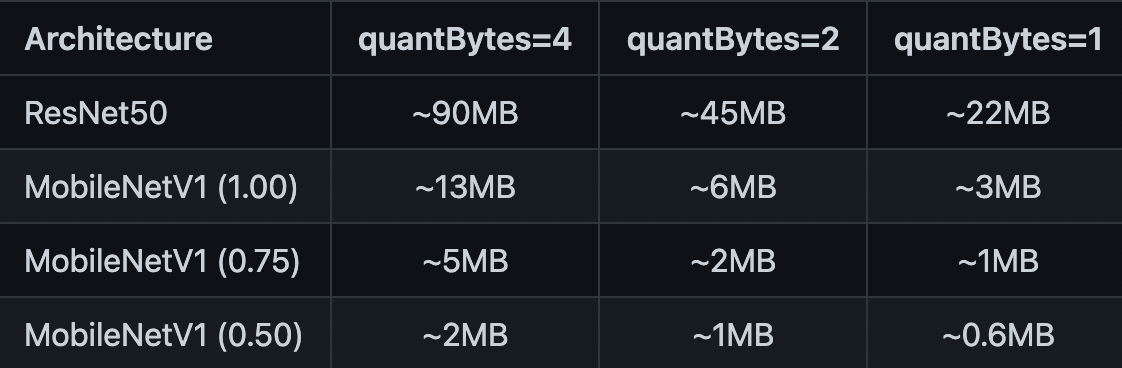
\includegraphics[width=13cm]{images/architectureTable.png}
\end{center}


However, the documentation specifies two recommended configurations for loading the model:
\begin{itemize}
    \item ResNet (larger, slower, more accurate):

    \begin{lstlisting}
    const model = await bodyPix.load({architecture: 'ResNet50',
                                      outputStride: 32,
                                      quantBytes: 2});

    \end{lstlisting}
    \item MobileNet (smaller, faster, less accurate):
    \begin{lstlisting}
    const model = await bodyPix.load({architecture: 'MobileNetV1',
                                      outputStride: 16,
                                      multiplier: 0.75,
                                      quantBytes: 2});
    \end{lstlisting}
\end{itemize}
The \textbf{second model} managed to have the fastest prediction in our application: 44 s. This is more than 40 times slower than our second experiment (approx. 1 second per prediction). Based on the table regarding the architecture we have also tried implementing the other configurations without having any success in obtaining a faster prediction (only values with a minimum of 50 seconds). 


Undoubtedly, this is the point where our third experiment ended, because of the bad performance in terms of time. A reaction that takes more than 44 seconds for a speeding car could be even more dangerous than a lack of reaction. In other words, we must keep in mind that the faster the answer, the less threatened human lives are, and we want to minimize the risk as much as possible.


\chapter{Application (numerical validation)}
\label{chapter:application}



\section{Methodology}
\label{section:methodology}

\begin{itemize}
	\item What are criteria you are using to evaluate your method? 
	
	Since our approach is based on the pre-trained version of the COCO-SSD model, we performed our experiments having in mind three aspects: 
	
    - accuracy
    
    - runtime (time for processing)
    
    - feasibility of our application in the context of driving assistance field
    
    The reason behind this was to balance these three.
	\item What specific hypotheses does your experiment test? 
	
	Due to the COCO-SSD model being very general,it is less likely to break down when applied to new domains or unexpected inputs. As a result, we can assume that the model will perform well on our task of detecting pedestrians, vehicles and other participants to the traffic. Starting with this assumption, our aim is to identify how well we can apply these existing algorithms of pre-trained model to a known objects detection problem in order to integrate in an application that provides driving assistance support.
	\item What are the dependent and independent variables? 
	
	Independent variables: Pre-trained model, System environment
	Dependent variables: DataSets, program output
	
	\item What is the training/test data that was used, and why is it realistic or interesting? 
	
	Our dataset contains real time images taken from in-motion video footage, making up for a very realistic experience, perfectly tailored to a real time driving assistant application.
	
\end{itemize}

\section{Data}
\label{section:data}

For the dataset, we selected some subsets from the COCO datasets. We will dive in details below.

COCO refers to the "Common Objects in Context" dataset, the data on which the model was trained on. This collection of images is mostly used for object detection, segmentation, and captioning, and it consists of over 200k labeled images belonging to one of 90 different categories, such as "person," "bus," "zebra," and "tennis racket."

Features of the COCO dataset

    - Object segmentation with detailed instance annotations
    
    - Recognition in context
    
    - Superpixel stuff segmentation
    
    - Over 200’000 images of the total 330’000 images are labeled
    
    - 1.5 Mio object instances
    
    - 80 object categories, the “COCO classes”, which include “things” for which individual instances may be easily labeled (person, car, chair, etc.)
    
    - 91 stuff categories, where “COCO stuff” includes materials and objects with no clear boundaries (sky, street, grass, etc.) that provide significant contextual information.
    
    - 5 captions per image
    
    - 250’000 people with 17 different keypoints, popularly used for Pose Estimation


https://mmla.gse.harvard.edu/tools/coco-ssd-object-detector/


\section{Results}
\label{section:results}

Each algorithmically generated result, such as an object bounding box or segment, is stored separately in its own result struct. This singleton result struct must contains the id of the image from which the result was generated (a single image will typically have multiple associated results). Results for the whole dataset are aggregated in a single array. Finally, this entire result struct array is stored to disk as a single JSON file.

Our initial intuition was to take a look at the original benchmark of the author of COCO-SSD algorithm which was completed on the COCO dataset and was run on a Pascal Titan X. The COCO-SSD algorithm itself has multiple versions that are suited for specific usecases.

For the metrics used in comparison, we focused on AP (Average precision) which is a popular metric in measuring the accuracy of object detectors like Faster R-CNN, SSD, etc. Average precision computes the average precision value for recall value over 0 to 1. 

\subsection{Results for YOLOv3}
\label{subsection:results}

We present the results for the YOLOv3 using COCO dataset in the following figure:
\begin{center}
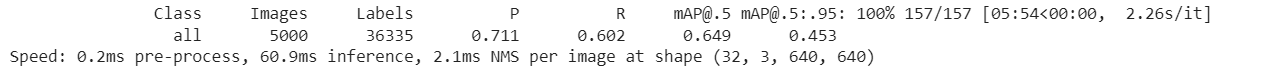
\includegraphics[width=16cm]{images/speed_yolo.PNG}   
Figure 5.3.1.1 Algorithm output for COCO dataset
\end{center}
\begin{center}
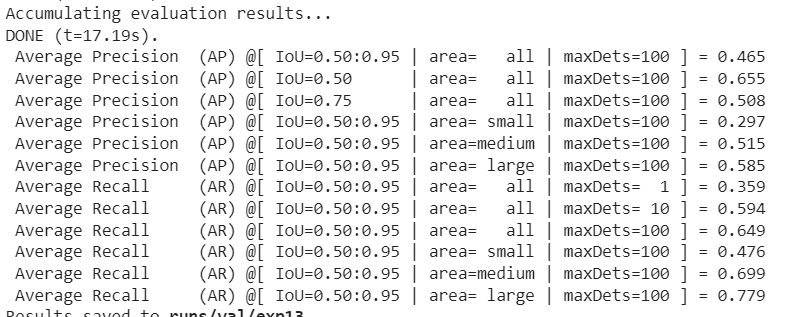
\includegraphics[width=16cm]{images/average precision yolo.PNG} 
Figure 5.3.1.2 Average precision for YOLOv3
\end{center}

Output images samples produced with YOLOv3:
\begin{center}
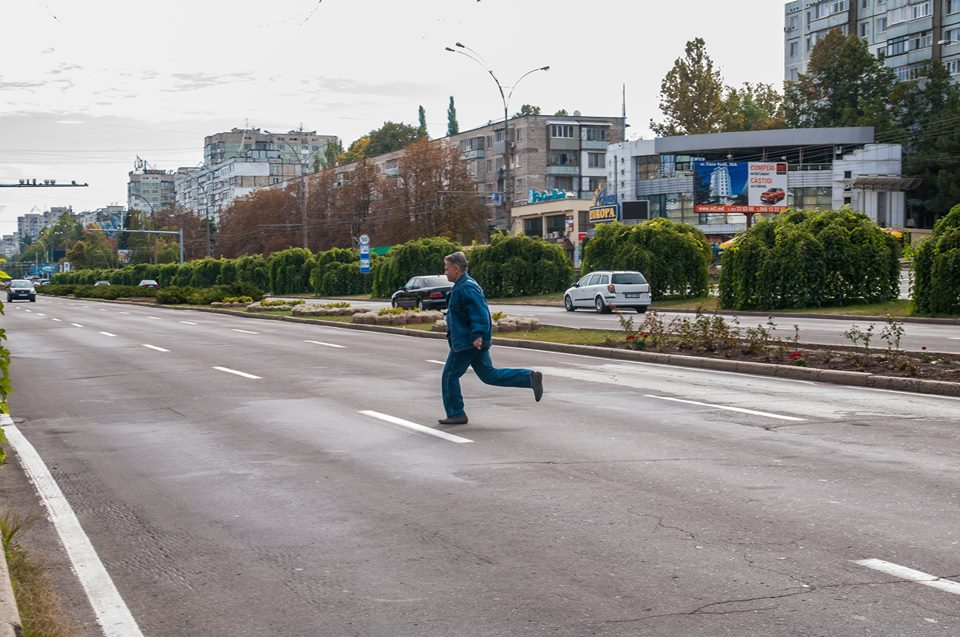
\includegraphics[width=8cm]{images/image1.png}   
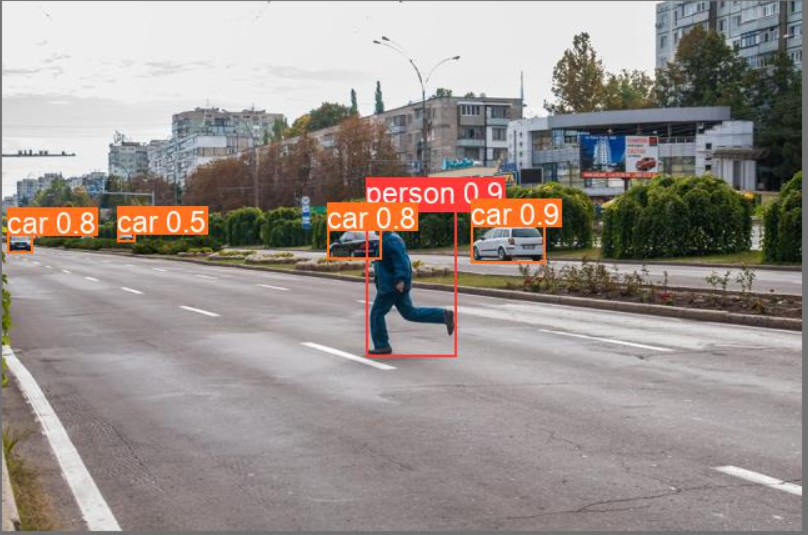
\includegraphics[width=8cm]{images/image1_label.PNG}
Figure 5.3.1.3 Output image sample for YOLOv3 1
\end{center}
\begin{center}
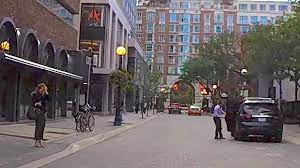
\includegraphics[width=8cm]{images/image2.jpg}   
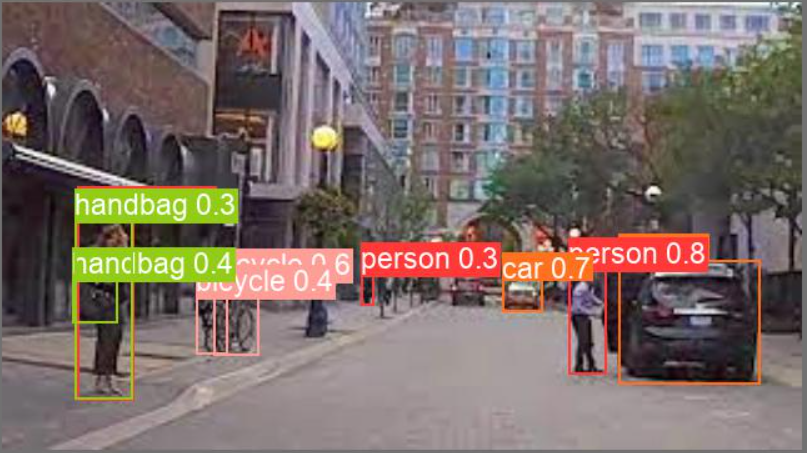
\includegraphics[width=8cm]{images/image2_label.PNG}
Figure 5.3.1.4 Output image sample for YOLOv3 2
\end{center}
\begin{center}
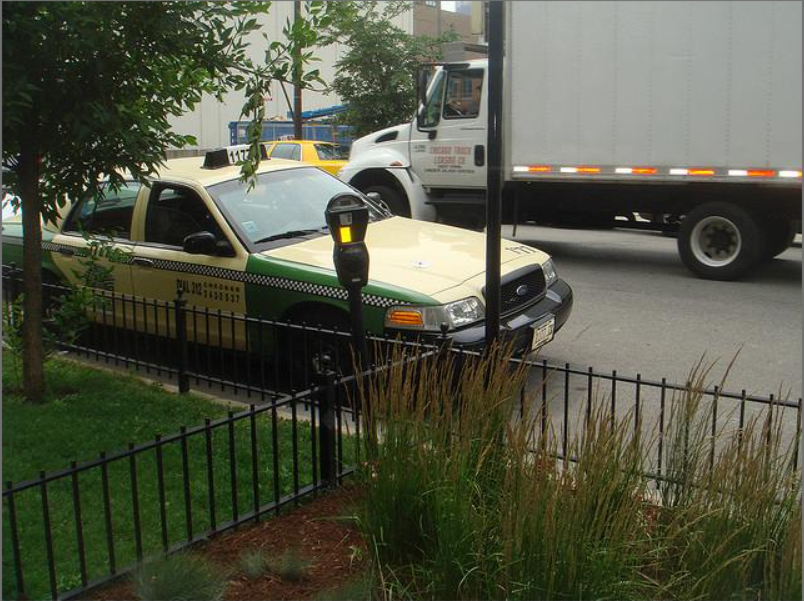
\includegraphics[width=8cm]{images/image3.png}   
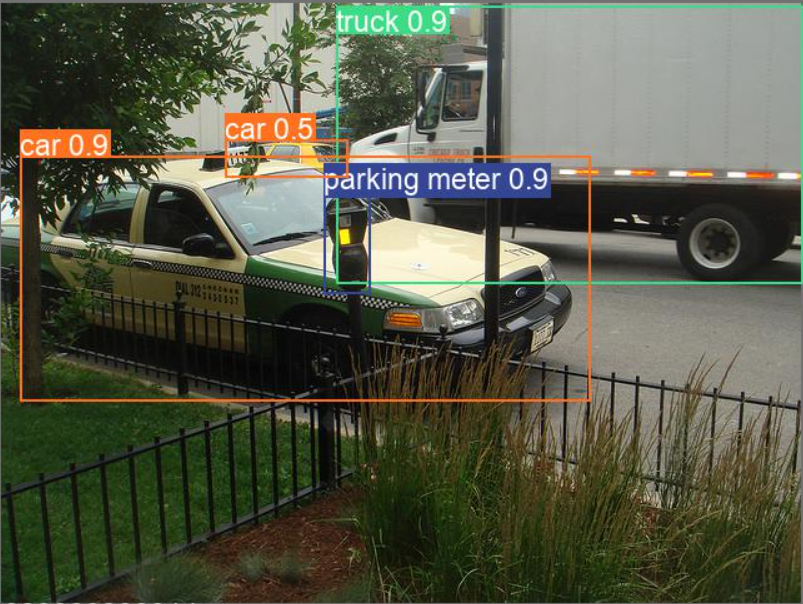
\includegraphics[width=8cm]{images/image3_label.PNG}
Figure 5.3.1.5 Output image sample for YOLOv3 3
\end{center}
\begin{center}
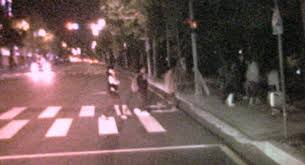
\includegraphics[width=8cm]{images/image4.jpg}   
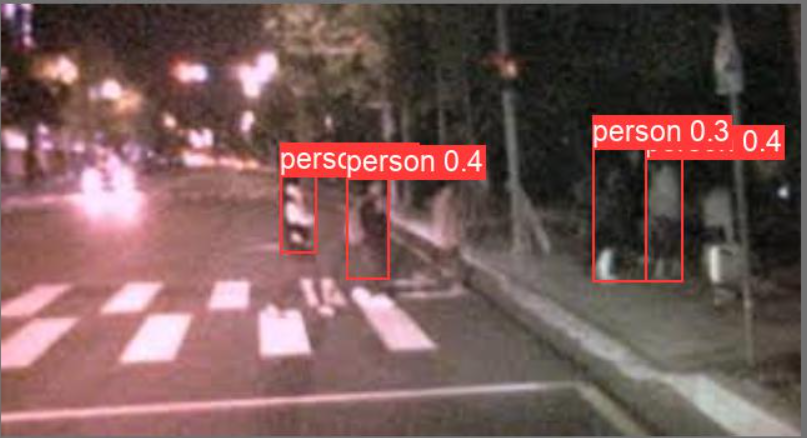
\includegraphics[width=8cm]{images/image4_label.PNG}
Figure 5.3.1.6 Output image sample for YOLOv3 4
\end{center}

 We observe that in general, the algorithm produces very good results and detects most of the pedestrians, vehicles and obstacles.
However, just like in the case of the smaller dataset, we notice the darker images will have a significantly lower precision than bright images (notice how in the Figure 5.3.1.6, the car is not detected and also some persons are not detected).

As s strong point for the algorithm, we could say that it manages to successfully tell apart trucks and larger vehicles of normal sized cars, and that means we can easily warn the driver of some imminent collision with a large vehicle to avoid an accident. (Figure 5.3.1.5)

\subsection{Results for COCO SSD in comparison with other models}
\label{subsection:results_coco}

TensorFlow 2 provides a collection of detection models pre-trained on the COCO 2017 dataset. The one we are using for mobile object detection has the following results:

\begin{center}
\begin{tabular}{||c c c c||} 
 \hline
 Model name & Speed (ms) & COCO mAP & Outputs \\ [0.5ex] 
 \hline\hline
 SSD MobileNet V2 FPNLite 320x320 & 22 & 22.2 & Boxes \\ 
 \hline
\end{tabular}
\end{center}
\begin{center}
Figure 5.3.2.1 Results on COCO dataset
\end{center}

https://github.com/tensorflow/models/blob/master/research/object_detection/g3doc/tf2_detection_zoo.md


Why have we chosen this backbone for our object detector? We believe that the crucial question is not the classical one regarding which detector is the best, as this might not be possible to answer. Instead, we are looking for the best balance between speed and accuracy that our problem needs.  

https://arxiv.org/pdf/1611.10012.pdf
A report conducted by Google Research offers a survey paper to study the tradeoff between \textbf{speed and accuracy} for Faster R-CNN, R-FCN, and SSD. The results show that SSD on MobileNet has the highest mAP among the models targeted for real-time processing, as Figure 5.3.2.2 shows:
\begin{center}
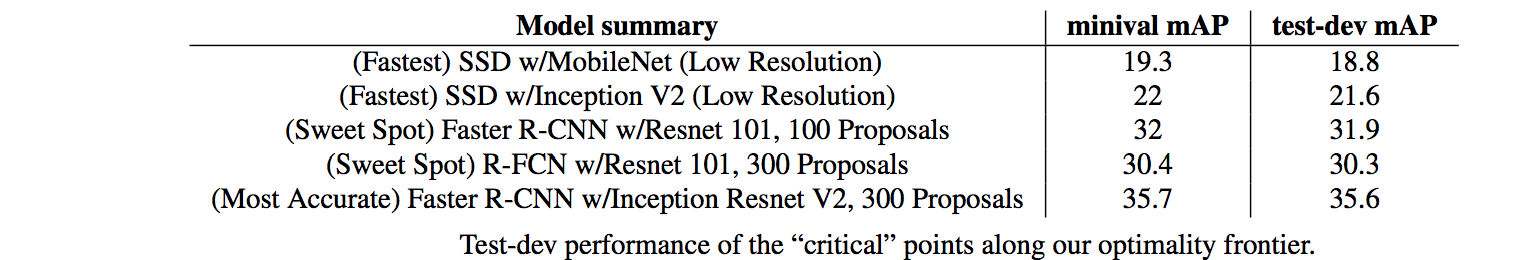
\includegraphics[width=17cm]{images/googleResearch.png}
Figure 5.3.2.2 mAP for Faster R-CNN, R-FCN, and SSD
\end{center}

On the other hand, since we are giving the model images as input, we should also refer to the \textbf{object size} when measuring the performance. For large objects, SSD performs pretty well even with a simple extractor. SSD can even match other detectors' accuracy using better extractor. But SSD performs much worse on small objects comparing to other methods. The following example is a screenshot from our application showing that no objects were detected by COCO SSD in a blurry picture with smaller objects, while, in our previous experiment, the objects were successfully detected by YOLO:

\begin{center}
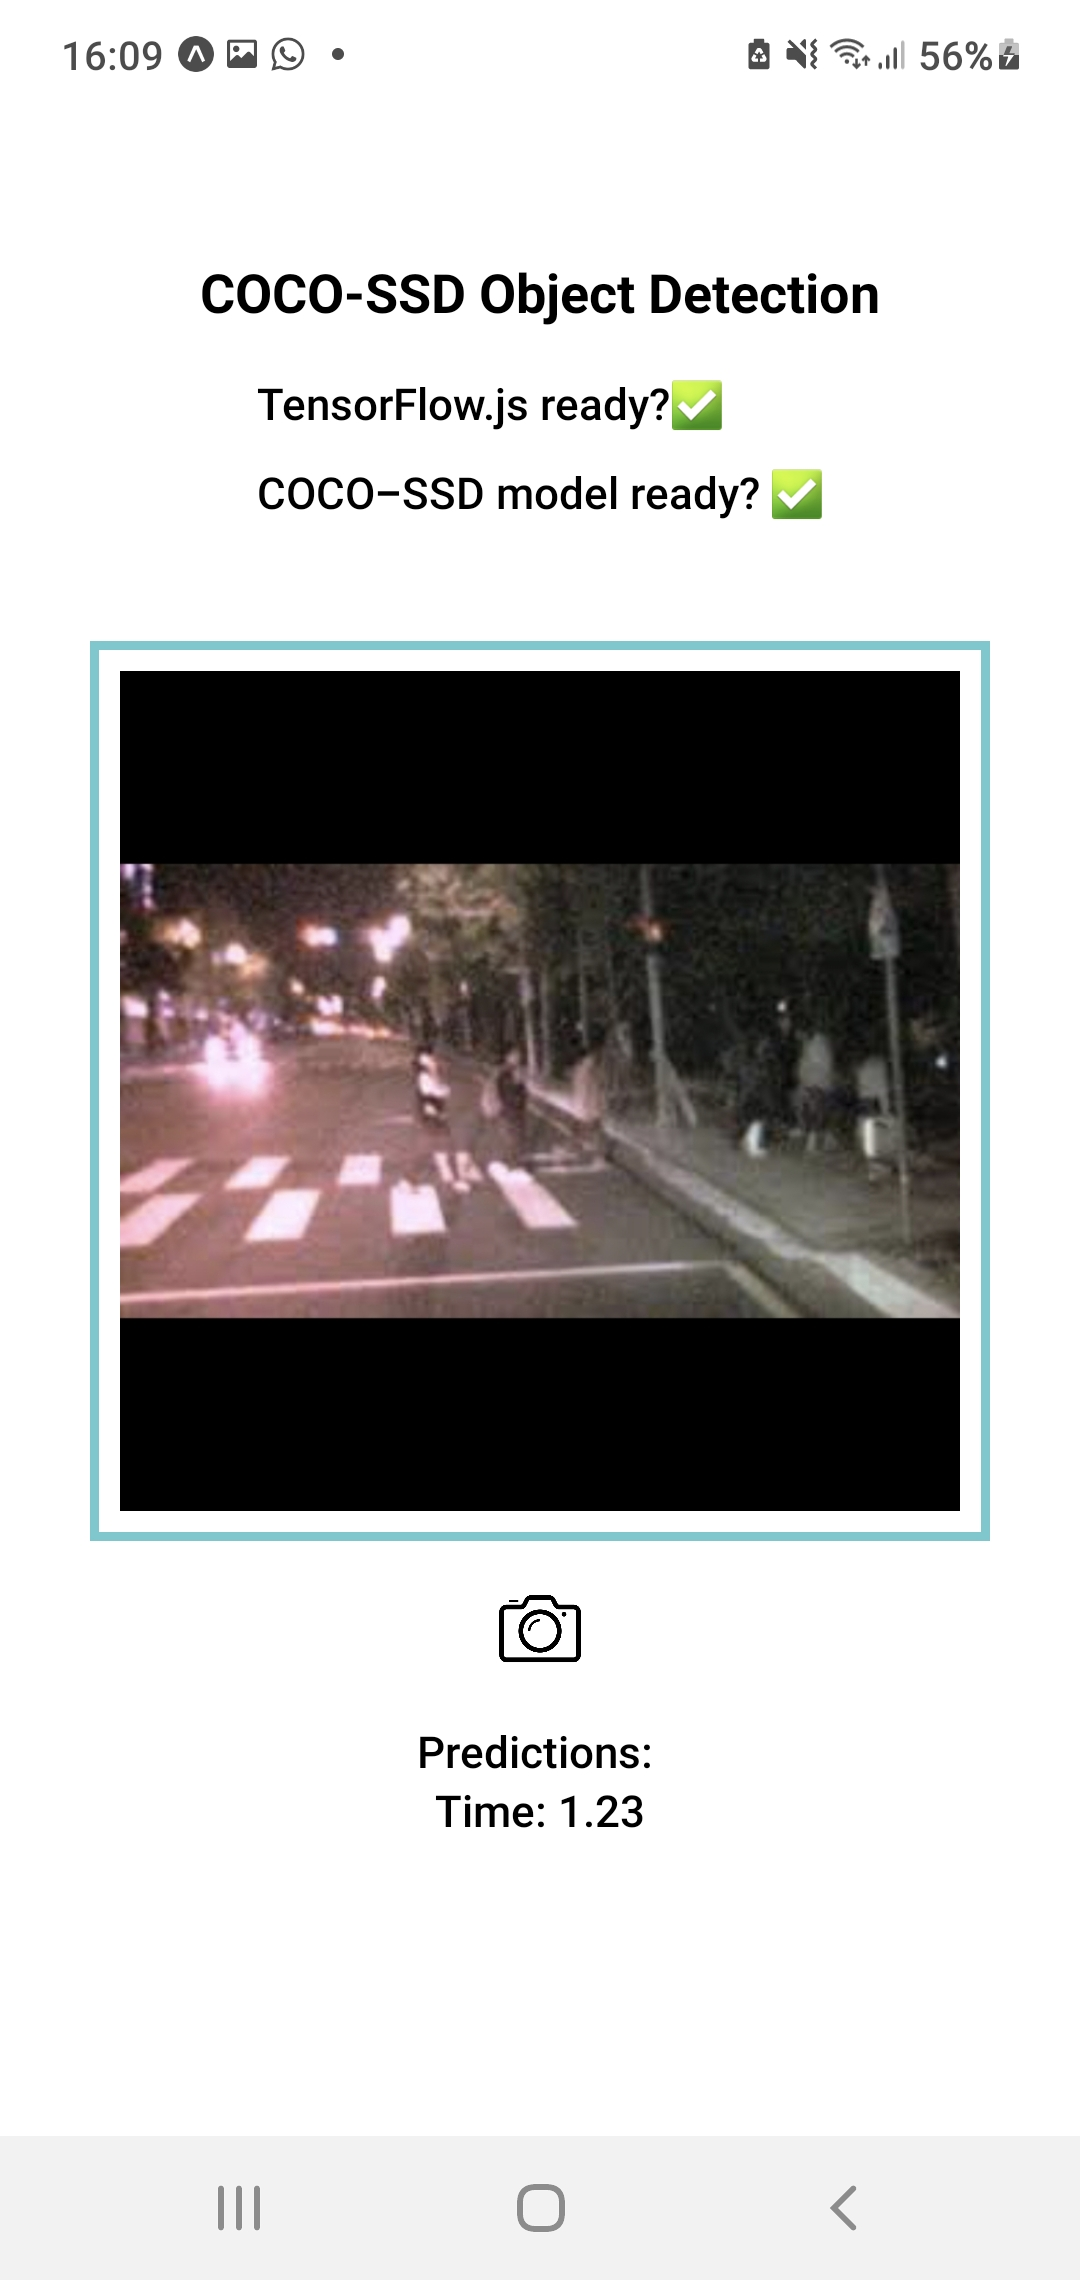
\includegraphics[width=8cm]{images/screenshot1.jpg}\\   
Figure 5.3.2.3 Output from COCO SSD for blurry, small objects
\break
\break
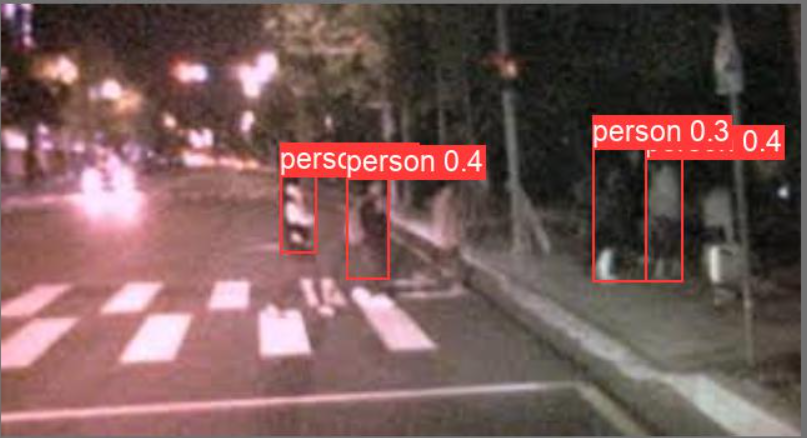
\includegraphics[width=8cm]{images/image4_label.PNG} \\
Figure 5.3.2.4 Output from YOLOv3 for blurry, small objects
\end{center}

At the same time, COCO SSD outperforms YOLOv3 in terms of \textbf{time}. Our application is designed to run on mobile, therefore it is not possible to store the model on the device, it needs to be accessed through an endpoint (REST server in our first experiment). For a clearer understanding of the matter, we propose a step by step list describing the process for running each of the two methods. \\
In order to make a prediction using YOLOv3, the following steps have to be pursued:
\begin{enumerate}
    \item rescale the image
    \item send it to the server
    \item decode the image
    \item run prediction
    \item encode the image
    \item send prediction response
\end{enumerate}
All these steps turned out to be very time consuming, as they all add a lot of overhead to the prediction task. Not to mention the cold start issue - when no request has been made to the server and the model is not loaded yet, loading it will take a few more seconds before running the actual prediction.
\\
In order to make the prediction using COCO SSD, TensorFlowJS is the fastest choice for mobile. The model is loaded once the app is first accessed, with no need for making a request for getting the predictions. Thus, the steps are:
\begin{enumerate}
    \item convert the image to string
    \item convert to tensor
    \item get prediction
\end{enumerate}
The pipeline is run on the client side entirely, with no other exhaustive and time consuming side tasks. Here are a couple of examples from after running COCO SSD on the mobile application:
\begin{center}
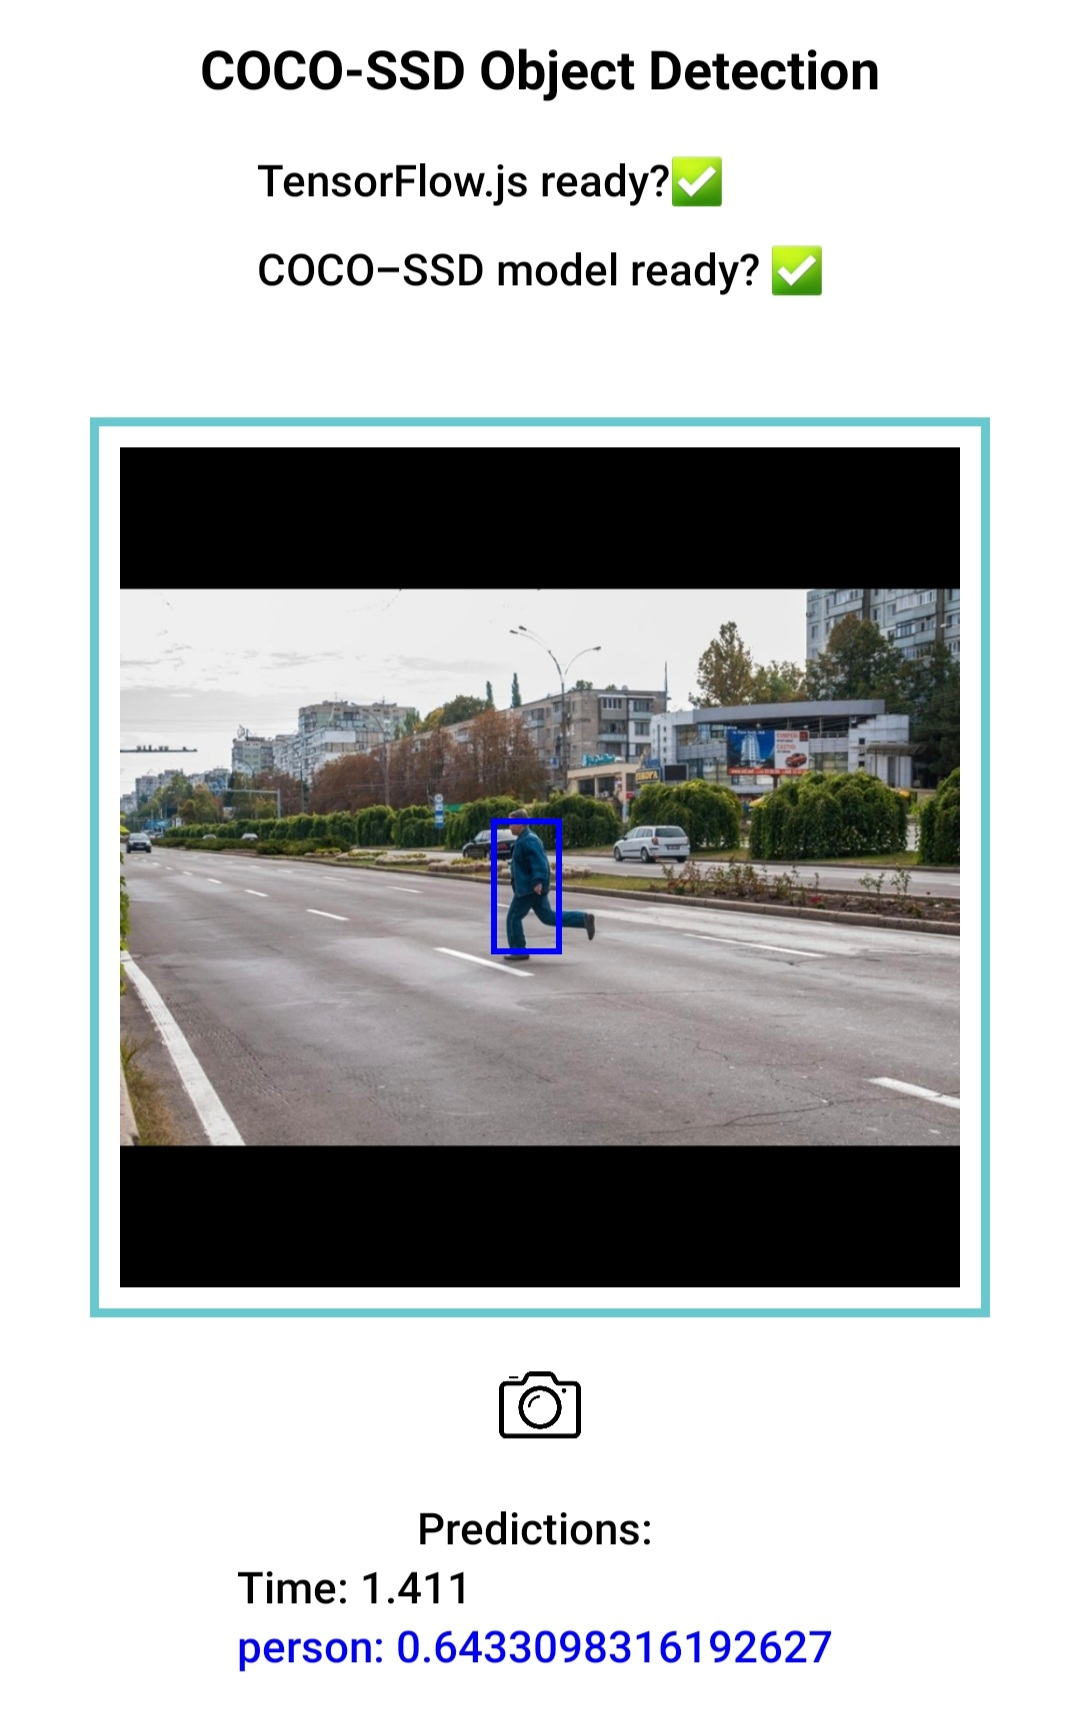
\includegraphics[width=7cm]{images/screenshot2.jpg}\\
Figure 5.3.2.5 COCO SSD prediction time example 1 - \textbf{COCO SSD: 1.4 (s) | YOLOv3: 5.32 (s)}
\break
\break
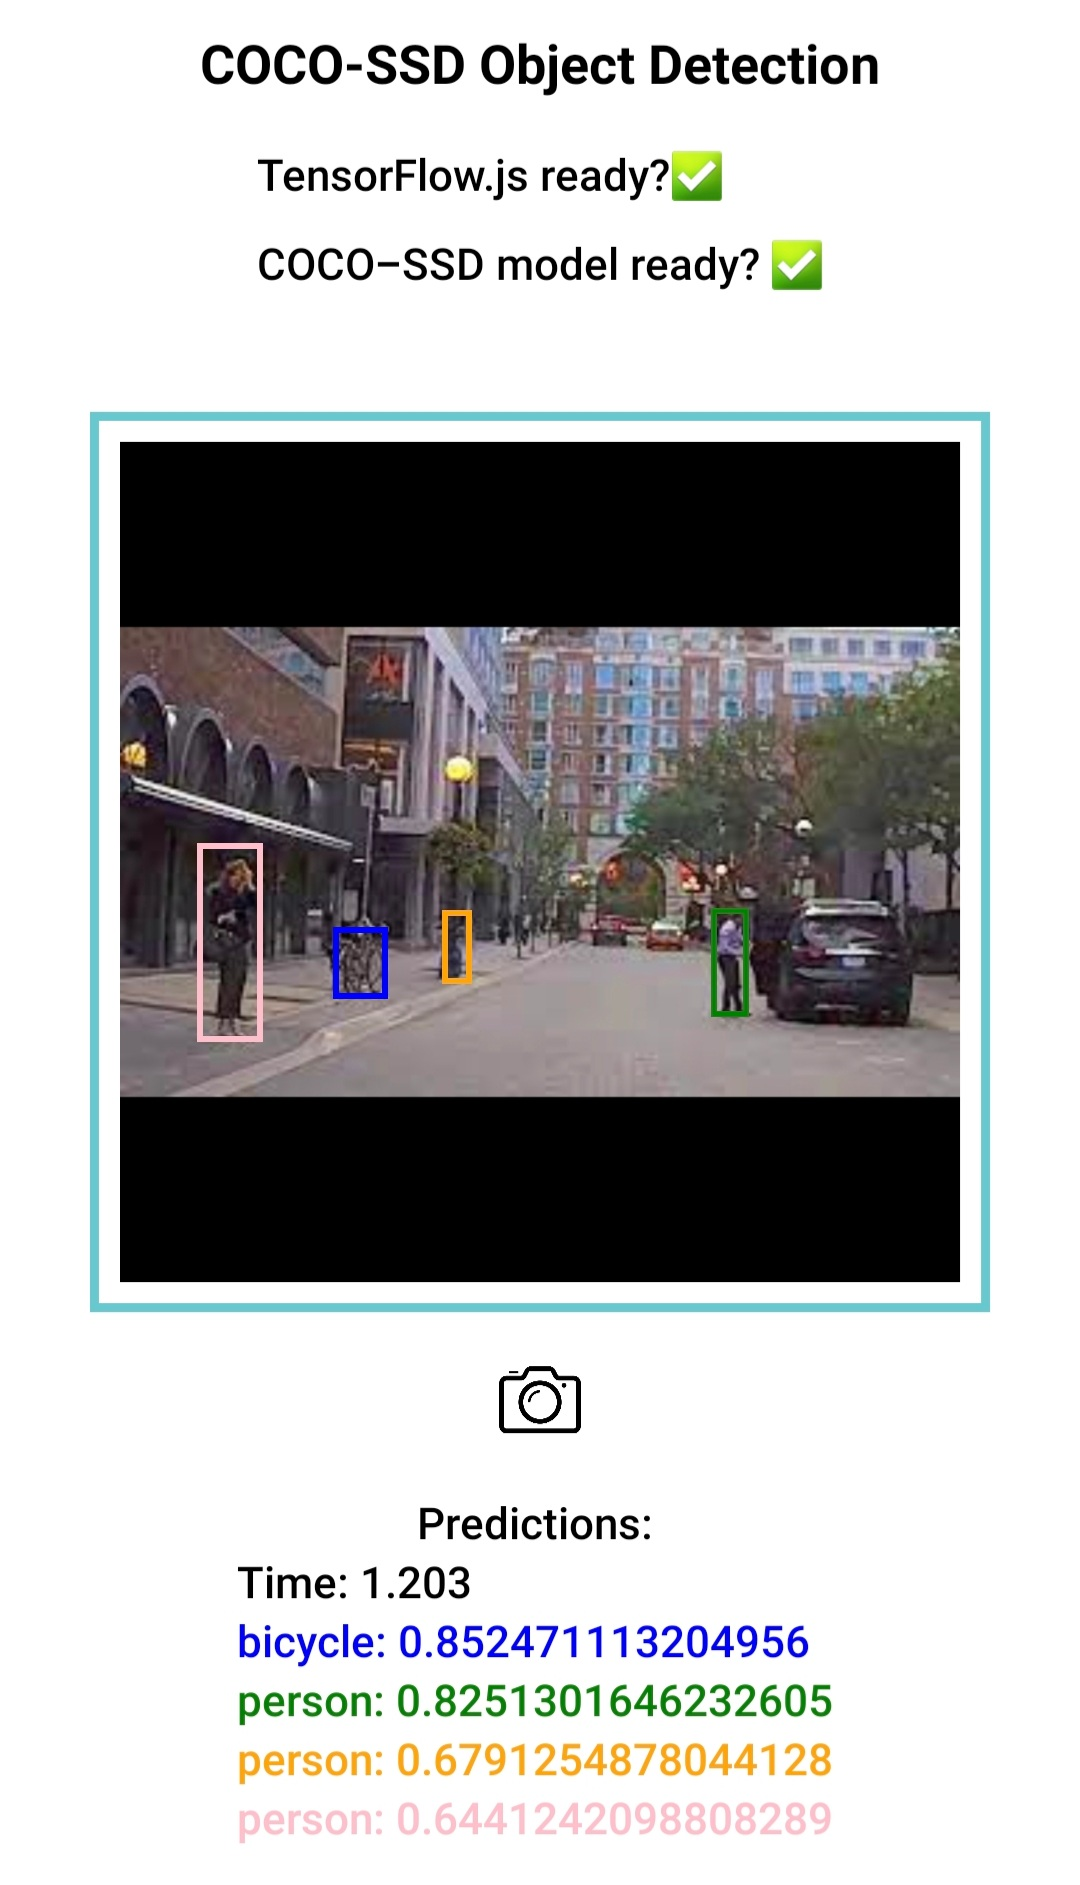
\includegraphics[width=7cm]{images/screenshot3.jpg}\\ 
Figure 5.3.2.6 COCO SSD prediction time example 2 - \textbf{COCO SSD: 1.2 (s) | YOLOv3: 4.7 (s)}
\end{center}
In the picture above (Figure 5.3.2.6), a very good result and also great performance from COCO SSD can easily be observed. The objects that are smaller have also successfully been detected here, as they are not blurry anymore (as in Figure 5.3.2.3). Moreover, the time difference between COCO SSD prediction using TensorFlowJS and YOLOv3 using a Python Flask REST server is huge - 4x the number of seconds that the SSD needs for the second option to get to the results. More details regarding the actual value of a millisecond in the context of driving will be described in the next section. 


\section{Discussion}
\label{section:discussion}

\begin{itemize}
	\item Is your hypothesis supported? 
	\item What conclusions do the results support about the strengths and weaknesses of your method compared to other methods? 
	At the first sight, the general impression is that YOLO is better than a SSD model. But we have to define what does actually better mean 
	\item How can the results be explained in terms of the underlying properties of the algorithm and/or the data. 
\end{itemize}


\chapter{Conclusion and future work}
\label{chapter:concl}

Try to emphasise the strengths and the weaknesses of your approach.
What are the major shortcomings of your current method? For each shortcoming, propose additions or enhancements that would help overcome it. 

Briefly summarize the important results and conclusions presented in the paper. 

\begin{itemize}
	\item What are the most important points illustrated by your work? 
	\item How will your results improve future research and applications in the area? 
\end{itemize}


\chapter{Latex examples}

Item example: 

\begin{itemize}
	\item content of item1
 	\item content of item2
 	\item content of item3
\end{itemize}



Figure example 

$\ldots$ (see Figure \ref{swarmsize})

\begin{figure}[htbp]
	\centerline{\includegraphics{Fig/FitEvol.eps}}  
	\caption{The evolution of the swarm size during the GA generations. This results were obtained for the $f_2$ test function with 5 dimensions.}
	\label{swarmsize}
\end{figure}


Table example: (see Table \ref{tab3PSO})


\begin{table}[htbp]
	\caption{The parameters of the PSO algorithm (the micro level algorithm) used to compute the fitness of a GA chromosome.}
	\label{tab3PSO}
		\begin{center}
			\begin{tabular}{p{220pt}c}

				\textbf{Parameter}& \textbf{Value} \\
				\hline\hline
 				Number of generations& 50 \\
 				Number of function evaluations/generation& 10 \\
 				Number of dimensions of the function to be optimized& 5 \\
 				Learning factor $c_{1}$& 2 \\
 				Learning factor $c_{2}$ & 1.8\\
 				Inertia weight& 0.5 + $\frac{rand()}{2}$\\
		
			\end{tabular}
		\end{center}
\end{table}

Algorithm example 

$\ldots$ (see Algorithm \ref{NGalg}).


\algsetup{indent=1em, linenosize=\footnotesize}

\begin{algorithm}
	\caption{SGA - Spin based Genetic AQlgorithm}
	\label{NGalg}
		\begin{algorithmic}


			\STATE \textbf{BEGIN}
  		\STATE @ Randomly create the initial GA population.
  		\STATE @ Compute the fitness of each individual.
  		\FOR{i=1 TO NoOfGenerations}
  			\FOR{j=1 TO PopulationSize}
  				\STATE p $\leftarrow$ RandomlySelectParticleFromGrid();
  				\STATE n $\leftarrow$ RandomlySelectParticleFromNeighbors(p);
  				\STATE @ Crossover(p, n, off);
  				\STATE @ Compute energy $\Delta H$
  				\IF {$\Delta H$ satisfy the Ising condition}
  					\STATE @ Replace(p,off);
  				\ENDIF
  			\ENDFOR
  		\ENDFOR
  		\STATE \textbf{END}
\end{algorithmic}
\end{algorithm}


\bibliographystyle{plain}
\bibliography{BibAll}

\end{document}
